\question Consider a \texttt{HashMap<Integer, String>} with an underlying array of size 5. Draw the resulting structure after the following operations. \texttt{Integer::hashCode} returns the integer's value itself.

\begin{lstlisting}
put(3, "monument");
put(8, "shrine");
put(3, "worker");
put(5, "granary");
put(13, "worker");
\end{lstlisting}

\ifprintanswers\else
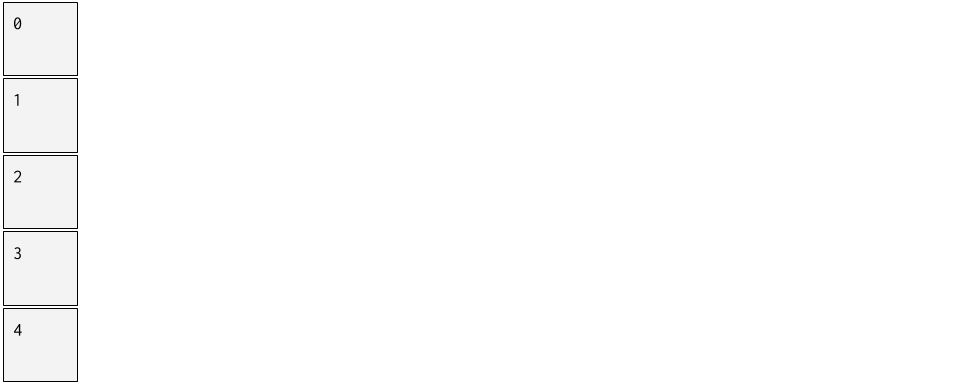
\includegraphics[width=\textwidth]{hashmap}
\fi

\begin{solution}
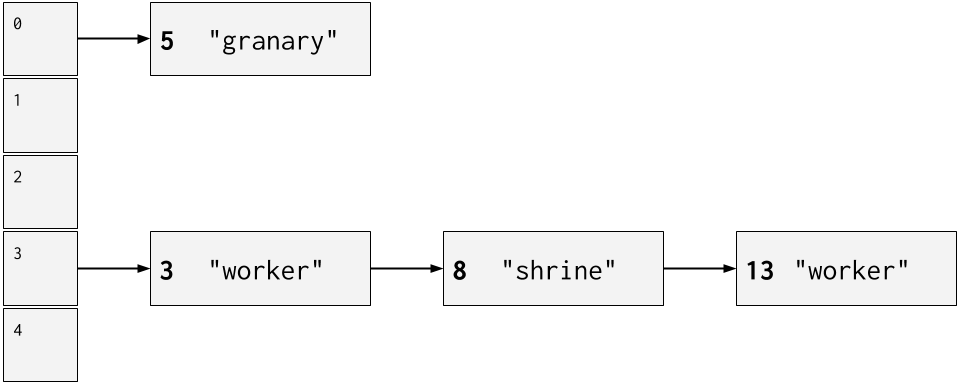
\includegraphics[width=\textwidth]{hashmap-sol}
\texttt{"worker"} replaces \texttt{"monument"} as their keys are the same. Each \texttt{put} must iterate through the entire external chain to ensure that a key-update is not necessary.
\end{solution}